% Name: Volume of revolution
% Description: The curve y = √x from 0 to 4 turned about the x-axis into a solid, with one disk of radius √x and thickness dx, and the volume the disk method gives.
% Tags: volume of revolution, disk method, solid of revolution, integral

\usetikzlibrary{arrows.meta}

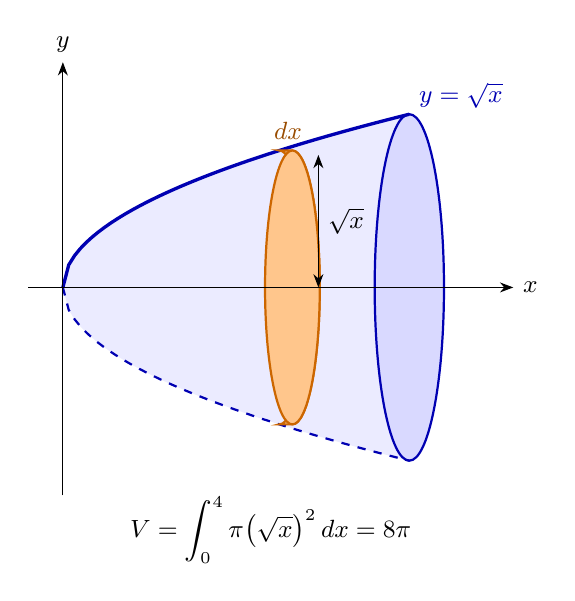
\begin{tikzpicture}[>={Stealth}, scale=1.1, every node/.style={font=\small}]
  % The solid's outline: the curve, its mirror image, and the circle at x = 4 seen at a slant
  \fill[blue!8] plot[domain=0:4, samples=60] (\x, {sqrt(\x)}) -- plot[domain=4:0, samples=60] (\x, {-sqrt(\x)}) -- cycle;
  \draw[thick, blue!70!black, fill=blue!15] (4,0) ellipse (0.4 and 2);
  \draw[very thick, blue!70!black, domain=0:4, samples=60] plot (\x, {sqrt(\x)});
  \draw[thick, blue!70!black, dashed, domain=0:4, samples=60] plot (\x, {-sqrt(\x)});
  % One disk at x = 2.5, radius √2.5 ≈ 1.581
  \draw[thick, orange!80!black, fill=orange!30] (2.5,-1.581) arc (-90:90:0.316 and 1.581) -- (2.65,1.581) arc (90:-90:0.316 and 1.581) -- cycle;
  \draw[thick, orange!80!black, fill=orange!45] (2.65,0) ellipse (0.316 and 1.581);
  \draw[->] (-0.4,0) -- (5.2,0) node[right] {$x$};
  \draw[->] (0,-2.4) -- (0,2.6) node[above] {$y$};
  \draw[<->, thin] (2.95,0) -- node[right] {$\sqrt{x}$} (2.95,1.53);
  \node[above, orange!60!black] at (2.6,1.6) {$dx$};
  \node[above right, blue!70!black] at (4,1.95) {$y = \sqrt{x}$};
  \node at (2.4,-2.8) {$\displaystyle V = \int_0^4 \pi\bigl(\sqrt{x}\bigr)^2\,dx = 8\pi$};
\end{tikzpicture}
